\chapter{従来手法を用いた足動作検知のためのBCI}
従来手法の枠組みによって構築した足動作検知のBCIについて説明する。
\section{計測したEEGについて}
まず、被験者が8秒間静止(以後rest状態)と
8秒間足動作(以後walk状態)を8サイクル繰り返したときのEEGを計測した。
被験者はリラックスできる椅子に着席した状態で前方に配置されたディスプレイの
指示に従って動作を行った(図\ref{fig:asibumi})。
ただし、8サイクル中最初の1サイクルについてはフィルタの応答の特性上、
EEGの解析には適さないと判断し、解析時には除外した。
従って以後の解析で用いられるのは7サイクル分のEEGである。
EEGの計測機器としてはg.tec社のg.USBamp(図\ref{fig:usbamp})を用い、ウェット式の電極を採用した。
ウェット式では頭皮と電極の間に導電性のジェルを注入することでEEGを計測する。
EEGの計測時にはジェルの注入を行いながら、すべての電極に関して電極インピーダンスが\(5k\Omega\)
以下になったことを確認した。
またサンプリング周波数は128Hzとした。
\begin{figure}
    \centering
    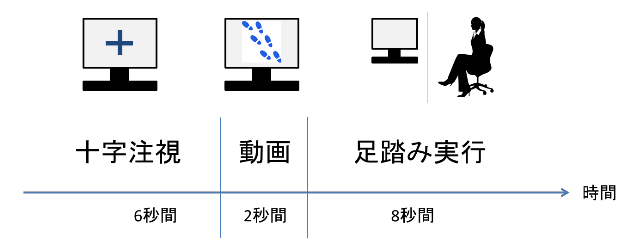
\includegraphics[width=13cm]{images/asibumi.png}
    \caption{EEG計測時のタイムスケジュール}
    \label{fig:asibumi}
\end{figure}
\begin{figure}
    \centering
    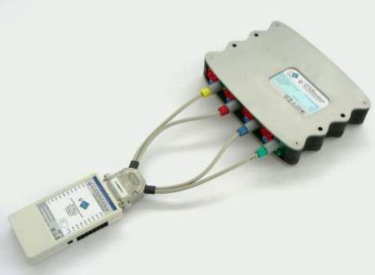
\includegraphics[width=8cm]{images/usbamp.png}
    \caption{g.tec社のg.USBamp}
    \label{fig:usbamp}
\end{figure}

計測に用いた電極の個数は5つであり、Cz、C1、C2、CPz、FCz電極である。
Cz電極は足に関する運動野が脳の頭頂部に存在するため選出し、
スモールラプラシアンフィルタが適用できるように残りの4つを選出した(図\ref{fig:smalllap})。
また、EEGの計測時には定常成分とERDとは無関係な高周波成分を削除するために
通過帯域を0.3Hzから36Hzとした2次のバタワースバンドパスフィルタを用いた。

\section{EEGの解析}
まずCz電極で計測されたEEGと
Cz電極に対してスモールラプラシアンフィルタを用いた際の
EEGを図\ref{fig:eegsub1}に添付する。
ここで、\(x_{A}(t)\)はA電極によって計測された波形であるとして
Cz電極に対してスモールラプラシアンフィルタを用いた際の波形\(z(t)\)は以下である。
\begin{equation}
    z(t) = x_{Cz}(t) - \frac{1}{4}(x_{C1}(t) + x_{C2}(t) + x_{FCz}(t) + x_{CPz}(t))
\end{equation}
スモールラプラシアンフィルタの定義から、
頭皮上でCz電極に際立った電位分布が獲得されていることが期待できる。

\begin{figure}
    \centering
    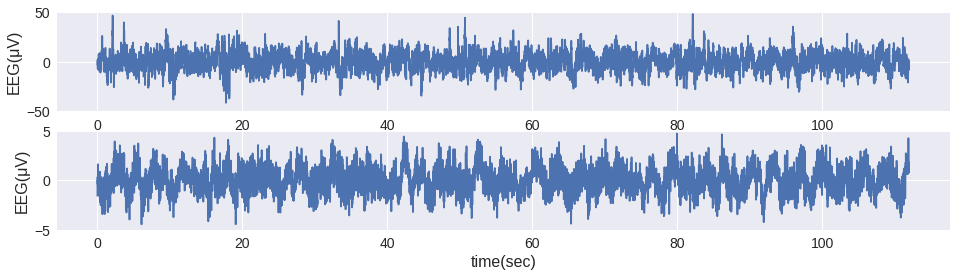
\includegraphics[width=13cm]{images/eeg_sub1.png}
    \caption{Cz電極のEEG(上)とスモールラプラシアンフィルタを用いたEEG(下)}
    \label{fig:eegsub1}
\end{figure}
% \begin{figure}
%     \centering
%     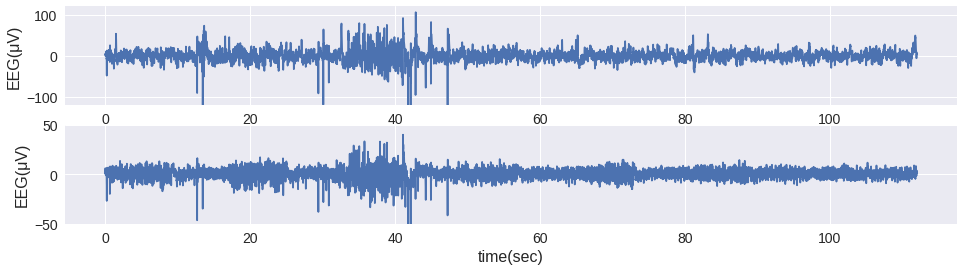
\includegraphics[width=13cm]{images/eeg_sub2.png}
%     \caption{被験者2のCz電極のEEG(上)とスモールラプラシアンフィルタを用いたEEG(下)}
%     \label{fig:eegsub2}
% \end{figure}

% 続いて、PCAとICAによる空間フィルタの設計を試みた。
% それぞれのフィルタから得られる各被験者のEEGの波形を図\ref{fig:bss1}と図\ref{fig:bss2}に示す。
% が\label{section:BSS}にて述べた問題のために、
% 得られた信号のいずれが重要であるかの判断を行うことができなかった。

次にスモールラプラシアンフィルタを用いたEEGの
rest状態(8秒間)の波形とwalk状態(8秒間)の波形それぞれに対してパワースペクトル密度推定を行った。
スペクトル密度推定には1秒間(128点)の時間窓を用いたウェルチのオーバラップ法を利用し、
オーバラップは0.5秒(64点)とした。
rest状態とwalk状態は計7回繰り返し行なっているため図\ref{fig:allERDs}に
7回分すべてのスペクトル密度の比較を示す。
また図\ref{fig:walkERD}に7回分の平均を示す。
ERDの生ずる周波数帯域は個人差があるとされるが、
\(\mu\)律動(8-12Hz)や\(\beta\)律動(18-26Hz)で
パワーの減少が観測できる報告があり\cite{erdfreq}、また\cite{Beta波によるBCI}では
6-40Hzの領域に渡ってERDを検知しBCIを構築した例がある。
概ね先行研究において観測されている周波数帯域でwalk時のパワーの減少が確認された。
\begin{figure}
    \centering
    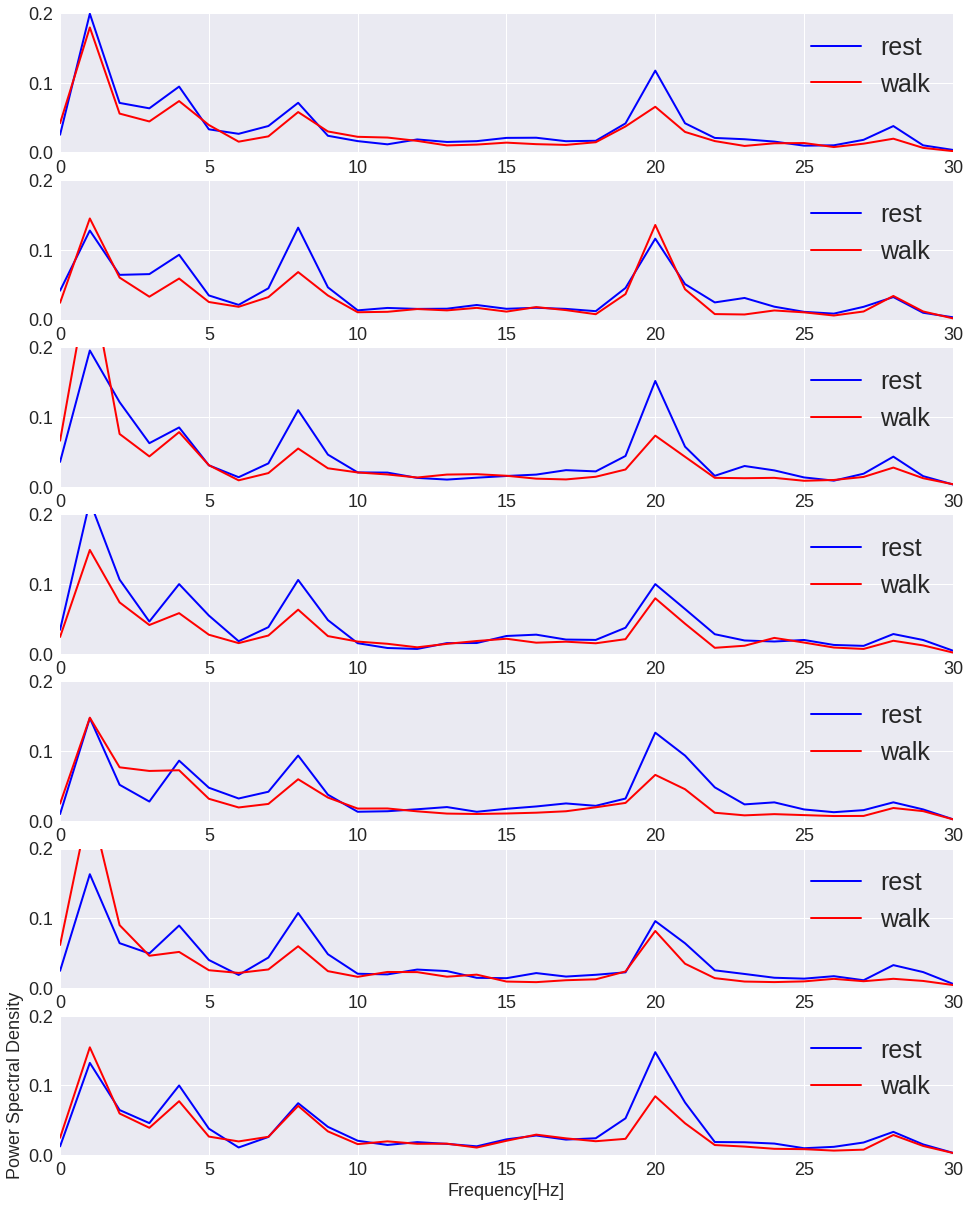
\includegraphics[width=13cm]{images/allERDs}
    \caption{rest時とwalk時のパワースペクトル密度の比較}
    \label{fig:allERDs}
\end{figure}
\begin{figure}
    \centering
    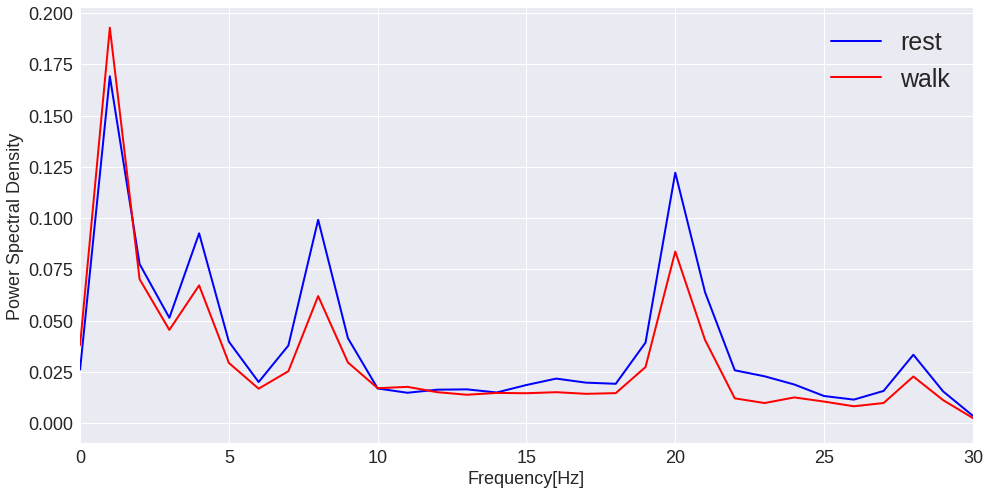
\includegraphics[width=13cm]{images/walkERD}
    \caption{rest時とwalk時のパワースペクトル密度の平均(7回分)の比較}
    \label{fig:walkERD}
\end{figure}

しかし、平均(図\ref{fig:walkERD})を確認すると
4、8、20Hz付近で際立ったパワーの減少が見られるが、
個々のスペクトル密度(図\ref{fig:allERDs})は必ずしもパワーの減少が
すべてのサイクルで同様に確認できることを示してはいない。
例として20Hzで際立ったパワーの減少(ERD)が生ずると考えた場合には、
図\ref{fig:allERDs}の上から2番目に関しては検知ができないことになる。
従って、ERDを検知してBCIを動作させることを考える場合には、
複数の周波数帯域のパワーを総合的に評価する必要があると考えられる。

また、パワースペクトル密度の絶対値を評価するよりも
rest状態とwalk状態の相対的なパワーの差の方が重要であることが言える。
例として、図\ref{fig:walkERD}から20Hzのパワースペクトル密度が0.1以下になった場合に
walk状態であると判定するBCIは図\ref{fig:allERDs}の下から二番目のグラフの
rest状態をwalk状態と判定することになる。
パワーの絶対値がさほど重要な指標にならないことは、
EEGの計測が電極のインピーダンス(ジェルの塗布状況)や
頭皮のインピーダンス(皮脂や毛髪)に左右されることからも想定されることである。

従ってERDを検知するためには複数の周波数帯域に跨って、
rest状態とwalk状態の相対的なパワーの変化に着目する必要があると考えた。


\subsection{足動作検知の信号処理}
解析結果に基づいて、EEGに対して以下の信号処理を構築した。
\begin{enumerate}
    \item 2種類のバンドパスフィルタ:通過帯域を3-14Hzと13-33Hz
    \item スモールラプラシアンフィルタ:Cz電極に適用
    \item バーグ法によるスペクトル密度推定:時間窓を1秒(128点)、オーバラップ127点
    \item ローパスフィルタ:スペクトル密度の時間変化の平滑化
    \item ハイパスフィルタ:パワースペクトル密度の時間変化の定常成分カット
\end{enumerate}
上記の処理における1.〜3.の概略図を図\ref{fig:footBCI}に示す。
\begin{figure}
    \centering
    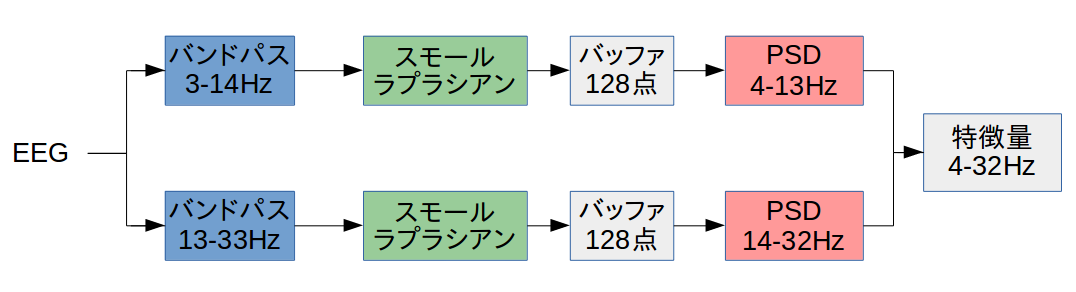
\includegraphics[width=13cm]{images/footBCI.png}
    \caption{EEGからスペクトル密度を獲得する処理の流れ}
    \label{fig:footBCI}
\end{figure}
1.〜3.の処理では2種類のバンドパスフィルタを通過したEEGに対してそれぞれスペクトル密度推定が行われる。
3−14Hzのバンドパスフィルタを通過した波形に関しては、パワースペクトル密度の4-13Hzのみを利用し、
13−33Hzのバンドパスフィルタを通過した波形に関しては、パワースペクトル密度の15-32Hzのみを利用した。
この着目する帯域は、EEGの\(\alpha\)律動及び\(\mu\)律動、\(\beta\)律動などの周波数帯域と
解析したEEGのピークの位置を加味し、経験的に定めた。
時間窓は1秒間であるため周波数分解能は1Hzであり、各時間窓において計28の特徴量が得られる。
時間窓は1サンプル点ずつ移動させるため、1/128秒毎に28次元の特徴量が出力される形となる。
図\ref{fig:nofilterERD}に1.〜3.の処理を施した出力を添付する。
\begin{figure}[p]
    \centering
    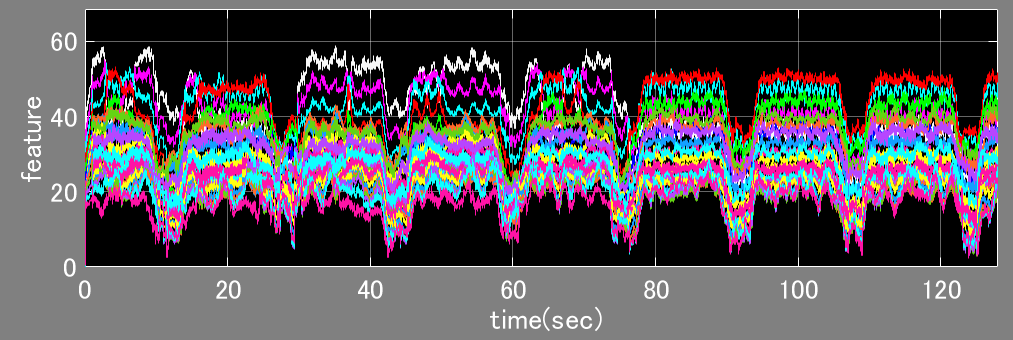
\includegraphics[width=13cm]{images/feature_sub1_nofilter.png}
    \caption{28個の特徴量の時間変化}
    \label{fig:nofilterERD}
\end{figure}
図\ref{fig:nofilterERD}では、
特徴量が全体的に減少している様子が8回分観測できる。
また特徴量はパワースペクトル密度の時間変化に他ならないため、
特徴量の減少はERDであり8回の足動作に由来していると考えられる。

次に、特徴量の変化がrest状態とwalk状態において際立つことが重要であり、
同一状態においては変化が少ない方が好ましいことを考慮し
4.ローパスフィルタによる平滑化を行った。この処理によって、
状態が切り替わる程の大きな特徴量の変化が強調される(図\ref{fig:lfilterERD})。
\begin{figure}[p]
    \centering
    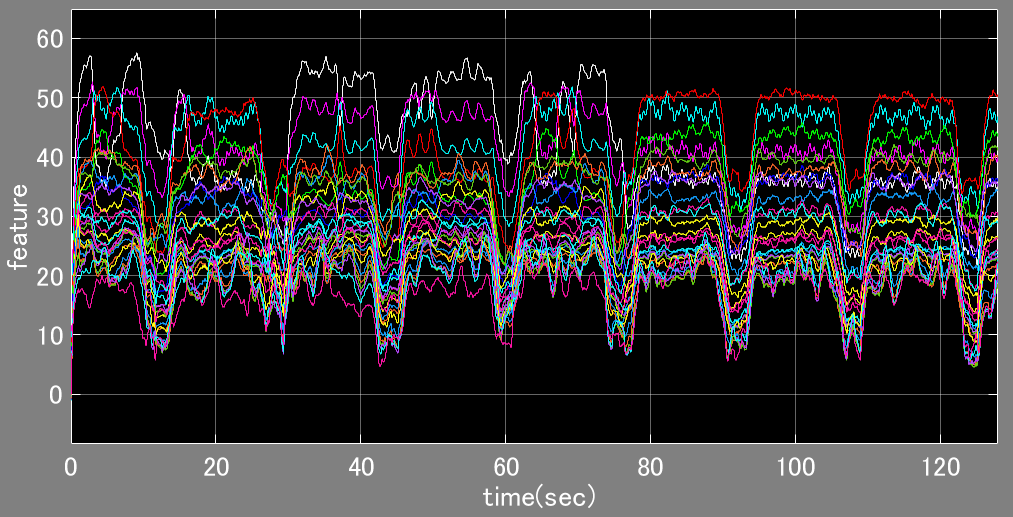
\includegraphics[width=13cm]{images/feature_sub1_l.png}
    \caption{ローパスフィルタを追加した28個の特徴量の時間変化}
    \label{fig:lfilterERD}
\end{figure}

また、ERDを検知する場合には
rest状態とwalk状態の各状態間のパワースペクトル密度の相対的差異が重要である
と考えられることを前述した。
同時に、分類機にとっても相対的差異のみが重要であり絶対値は影響しないことを考慮し、
5.ハイパスフィルタによって定常成分をカットした(図\ref{fig:filterERD})。

\begin{figure}[p]
    \centering
    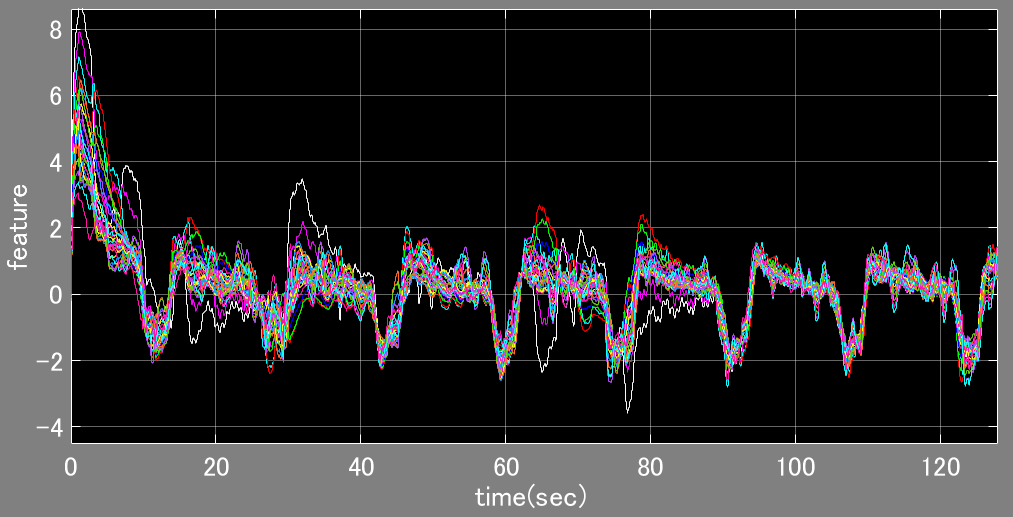
\includegraphics[width=13cm]{images/feature_sub1.png}
    \caption{ローパスフィルタとハイパスフィルタを追加した28個の特徴量の時間変化}
    \label{fig:filterERD}
\end{figure}